\section{Time Complexity}

  The Big O notation is a mathematical notation that describes the limiting behavior of a function when the argument tends towards a particular value of infinity. That is, if the time it takes for an algorithm to complete a problem with input size $n$ is given by $f(n)$, then we say that the computational complexity is of the \textit{order} $O(f(n))$. More formally, we can define it as such: 

  \begin{definition}[Big-O Notation]
    Let $f$ and $g$ be (nonnegative) real-valued functions both defined on the positive integers, and let $g(x)$ be strictly positive for all large enough values of $x$. One writes
    \[f(x) = O\big( g(x)\big) \text{ as } x \rightarrow \infty\]
    if the absolute value of $f(x)$ is at most a positive constant multiple of $g(x)$ for all sufficiently large values of $x$. That is, $f(x) = O \big(g(x)\big)$ if there exist positive integers $M$ and $n_0$ such that
    \[f(n) \leq M g(n) \text{ for all } n \geq n_0\]
    In many contexts, the assumption that we are interested in the growth rate as the variable $x$ goes to infinity is left unstated, and one write more simply that
    \[f(x) = O\big( g(x)\big)\]
  \end{definition}

  \begin{example}[Simple Runtime Calulation for Polynomials]
    Let there be a program that given input with length $x$, takes $f(x) = 6x^4 - 2x^3 + 5$ steps to solve whatever problem needs to be solved. Then, using the simplification steps above, we have 
    \begin{equation}
      f(x) = O(x^4)
    \end{equation}
  \end{example}

  When talking about running time, what we care about is the \textit{scaling behavior} of the number of steps as the input size grows (as opposed to a fixed number). 

\subsection{Formally Defining Running Time}

  We can informally define what it means for a function $F: \{0,1\}^* \longrightarrow \{0,1\}^*$ to be \textit{computable} in time $T(n)$ steps, where $T$ is some function mapping the length $n$ of the input to the number of computation steps allowed. 

  \begin{definition}
  Let $T: \mathbb{N} \longrightarrow \mathbb{N}$ be some function. We say that a function $F: \{0,1\}^* \longrightarrow \{0,1\}^*$ is \textbf{computable in $T(n)$ Turing Machine time (TM-time for short)} if there exists a Turing machine $M$ such that for every sufficiently large $n$ and every $x \in \{0,1\}^n$, the machine halts after executing at most $T(n)$ steps and outputs $F(x)$. 

  We define $TIME_{\mathsf{TM}}\big(T(n)\big)$ to be the set of Boolean functions ($\{0,1\}^* \longrightarrow \{0,1\}$) that are computable in $T(n)$ TM time. Note that $TIME_{\mathsf{TM}}\big(T(n)\big)$ is a class of \textit{functions}, not machines. 
  \end{definition}

  With this, we can formally define what is means for function $F: \{0,1\}^* \longrightarrow \{0,1\}$ to be computable in time at most $T(n)$ where $n$ is the size of the input. Furthermore, the property of considering only "sufficiently large" $n$'s is not very important but it is convenient since it allows us to avoid dealing explicitly with uninteresting "edge cases." We have also defined computability with Boolean functions for simplicity, but we can generalize this further. 

\subsubsection{Polynomial and Exponential Time}

  \begin{definition}
    A \textbf{decision problem} is a problem that can be posed as a yes-no question on an infinite set of inputs. A method for solving a decision problem, given in the form of an \textit{algorithm}, is called a \textbf{decision procedure} for that problem. A decision problem which can be solved by an algorithm is called \textbf{decidable}. 
  \end{definition}

  It is traditional to define the decision problem as the set of possible inputs together with the set of inputs for which the answer is yes, and the set of inputs (i.e. the domain) can be numbers, floats, strings, etc. 

  \begin{example}
    Two examples of decision problems are: 
    \begin{enumerate}
      \item Deciding whether a given natural number is prime. 
      \item Given two numbers $x$ and $y$, does $x$ evenly divide $y$? The decision procedure can be long division. 
    \end{enumerate}
  \end{example}

  \begin{definition}
  The two main time complexity classes are defined: 
  \begin{enumerate}
      \item \textbf{Polynomial time}: A function $F: \{0,1\}^* \longrightarrow \{0,1\}$ is \textbf{computable in polynomial time} if it is in the class
      \[\mathbf{P} = \bigcup_{c \in \{1, ...m\}} TIME_{\mathsf{TM}} \big( n^c \big), \;\;\; m \in \mathbb{N}\]
      That is, $F \in \mathbf{P}$ if there is an algorithm to compute $F$ that runs in time at most \textit{polynomial} in the length of the input. 
      \item \textbf{Exponential time}: A function $F: \{0,1\}^* \longrightarrow \{0,1\}$ is \textbf{computable in exponential time} if it is in the class 
      \[\mathbf{EXP} = \bigcup_{c \in \{1, ..., m\}} TIME_{\mathsf{TM}} \big( 2^{n^c}\big)\]
      That is, $F \in \mathbf{EXP}$ if there is an algorithm to compute $F$ that runs in time at most \textit{exponential} in the length of the input. 
  \end{enumerate}
  Summarizing this, we say that $F \in \mathbf{P}$ if there is a polynomial $p: \mathbb{N} \longrightarrow \mathbb{R}$ and a Turing machine $M$ such that for every $x \in \{0,1\}^*$, when given input $x$, the Turing machine halts within at most $p(|x|)$ steps and outputs $F(x)$. 

  We say that $F \in \mathbf{EXP}$ if there is a polynomial $p: \mathbb{N} \longrightarrow \mathbb{R}$ and a Turing machine $M$ such that for every $x \in \{0,1\}^*$, when given input $x$, $M$ halts within at most $2^{p(|x|)}$ steps and outputs $F(x)$. 
  \end{definition}

  \begin{lemma}
  Since exponential time is much larger than polynomial time, 
  \[\mathbf{P} \subset \mathbf{EXP}\]
  \end{lemma}

  Time complexity for the previous algorithms are as follows: 
  \begin{center}
  \begin{tabular}{l|l}
      \textbf{P} & \textbf{EXP} (not known to be \textbf{P}) \\
      \hline
      Shortest path & Longest path \\
      Min cut & Max cut \\
      2SAT & 3SAT \\
      Linear eqs & Quad eqs \\
      Zerosum & Nash \\
      Determinant & Permanent\\
      Primality & Factoring
  \end{tabular}
  \end{center}
  Many technological developments are centered around these facts. For example, the exponential time complexity of factoring algorithms is what makes the RSA-encryption so secure. If a polynomial time algorithm for factoring were to be discovered, RSA-encryption would be rendered obsolete. 

\subsection{Modeling Running Time Using RAM Machines/NAND-RAM}

  Despite the theoretical elegance of Turing machines, RAM machines and NAND-RAM programs are much more closely related to actual computing architecture. For example, even a "merge sort" program cannot be implemented on a Turing machines in $O(n \log n)$ time. We can define running time with respect to NAND-RAM programs just as we did for Turing machines. 

  \begin{definition}
  Let $T: \mathbb{N} \longrightarrow \mathbb{N}$. We say that a function $F: \{0,1\}^* \longrightarrow \{0,1\}^*$ is \textbf{computable in $\mathbf{T(n)}$ RAM time (RAM-time for short)} if there exists a NAND-RAM program $P$ such that for every sufficiently large $n$ and every $x \in \{0,1\}^n$, when given input $x$, the program $P$ halts after executing at most $T(n)$ lines and outputs $F(x)$. 

  We define $TIME_{\mathsf{RAM}} \big(T(n)\big)$ to be the set of Boolean functions ($\{0,1\}^* \longrightarrow \{0,1\}$) that are computable in $T(n)$ RAM time. 
  \end{definition}

  We will use $TIME \big( T(n)\big)$ to denote $TIME_{\mathsf{RAM}} \big(T(M) \big)$. However, as long as we only care about the difference between exponential and polynomial time, the model of running time we use does not make much difference. The reason is that Turing machines can simulate NAND-RAM programs with at most a polynomial overhead. 

  \begin{theorem}[Relating RAM and Turing machines]
  Let $T: \mathbb{N} \longrightarrow \mathbb{N}$ be a function such that $T(n) \geq n$ for every $n$ and the map $n \mapsto T(n)$ can be computed by a Turing machine in time $O(T(n))$. Then, 
  \[TIME_{\mathsf{TM}}\big( T(n)\big) \subseteq TIME_{\mathsf{RAM}}\big( 10 \cdot T(n)\big) \subseteq TIME_{\mathsf{TM}} \big( T(n)^4\big)\]
  We can visually see this classification as 
  \begin{center}
  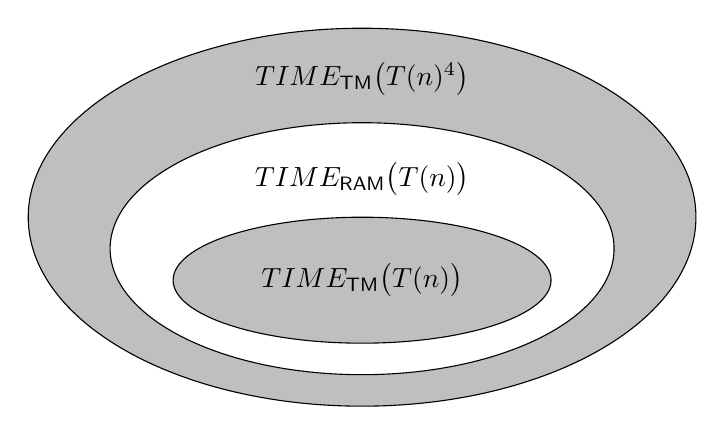
\begin{tikzpicture}[scale=0.8]
      \draw[fill=lightgray] (0,1) ellipse (5.3 and 3);
      \draw[fill=white] (0,0.5) ellipse (4 and 2);
      \draw[fill=lightgray] (0,0) ellipse (3 and 1);
      \node at (0,0) {$TIME_{\mathsf{TM}}\big(T(n)\big)$};
      \node at (0,1.6) {$TIME_{\mathsf{RAM}}\big(T(n)\big)$};
      \node at (0,3.2) {$TIME_{\mathsf{TM}}\big(T(n)^4\big)$};
  \end{tikzpicture}
  \end{center}
  \end{theorem}

  With this, we could have equally defined $\mathbf{P}$ as the class of functions computable by NAND-RAM programs (instead of Turing machines) that run in polynomial time in the length of the input. Similarly, with $T(n) = 2^{n^a}$, we see that the class $\mathbf{EXP}$ can also be defined as the set of functions computable by NAND-RAM programs in time at most $2^{p(n)}$ where $p$ is some polynomial. This justifies the choice of $\mathbf{P}$ as capturing a technology-independent notion of tractability. Therefore, \textit{all "reasonable" computational models are equivalent if we only care about the distinction between polynomial and exponential}, with reasonable referring to all scalable computational models that have been implemented except possibly quantum computers. 

  When considering general time bounds, we need to make sure to rule out some "exceptional" cases such as functions $T$ that don't give enough time for the algorithm to even read the input, or functions where the time bound itself is uncomputable. More precisely, $T$ must be a \textit{nice function}. 

  \begin{definition}
  That is why we say that the function $T: \mathbb{N} \longrightarrow \mathbb{N}$ is a \textbf{nice time bound function} (\textbf{nice function} for short) if 
  \begin{enumerate}
      \item for every $n \in \mathbb{N}$ $T(n) \geq n$ ($T$ allows enough time to read the input)
      \item for every $n^\prime \geq n$, $T(n^\prime) \geq T(n)$ ($T$ allows more time on longer inputs)
      \item the map $F(x) = 1^{T(|x|)}$ (i.e. mapping a string of length $n$ to a sequence of $T(n)$ ones) can be computed by a NAND-RAM program in $O(T(n))$ time
  \end{enumerate}
  \end{definition}

  So, the following are examples of polynomially equivalent models: 
  \begin{enumerate}
      \item Turing machines
      \item NAND-RAM programs/RAM machines
      \item All standard programming languages, including C/Python/Javascript...
      \item The $\lambda$ calculus
      \item Cellular automata
      \item Parallel computers
      \item Biological computing devices such as DNA-based computers 
  \end{enumerate}

  The \textit{Extended Church Turing Thesis} is the statement that this is true for all physically realizable computing models. In other words, the extended Church Turing thesis says that for every \textit{scalable computing device} $C$ (which has a finite description but can be in principle used to run computation on arbitrarily large inputs), there is some constant $a$ such that for every function $F: \{0,1\}^* \longrightarrow \{0,1\}$ that $C$ can compute on $n$ length inputs using an $S(n)$ amount of physical resources. This is a strengthening of the plain Church Turing Thesis, which states that the set of computable functions is the same for all physically realizable models, but without requiring the overhead in the simulation between different models to be at most polynomial. 

  Like the Church-Turing thesis itself, the extended Church-Turing thesis is in the asymptotic setting and does not directly yield an experimentally testable prediction. However, it can be instantiated with more concrete bounds on the overhead, yielding experimentally- testable predictions such as the Physical Extended Church-Turing Thesis. 
   
\subsection{Efficient Universal Machine: A NAND-RAM Interpreter in NAND-RAM}

  We can now see that the universal Turing machine $U$, which can compute every Turing machine $M$, has a \textit{polynomial} overhead for simulating a $NAND-TM$ program. That is, it can simulate $T$ steps of a given $NAND-TM$ (or $NAND-RAM$) program $P$ on an input $x$ in $O(T^4)$ steps. But in fact, by directly simulating $NAND-RAM$ programs we can do better with only a \textit{constant} multiplicative overhead. 

  \begin{theorem}[Efficient Universality of NAND-RAM]
  There exists a NAND-RAM program $U$ satisfying the following: 
  \begin{enumerate}
      \item \textit{U is a universal NAND-RAM program}: For every NAND-RAM program $P$ and input $x$, $U(P, x) = P(x)$ where by $U(P, x)$ we denote the output of $U$ on a string encoding the pair $(P, x)$. 
      \item \textit{U is efficient}: There are some constants $a, b$ such that for every $NAND-RAM$ program $P$, if $P$ halts on input $x$ after most $T$ steps, then $U(P, x)$ halts after at most $C \cdot T$ steps where $C \leq a |P|^b$. 
  \end{enumerate}
  \end{theorem}

  This leads to a corollary. Given any Turing machine $M$, input $x$, and \textit{step budget} $T$, we can simulate the execution for $M$ for $T$ steps in time that is polynomial in $T$. Formally, we define a function $TIMEDEVAL$ that takes the three parameters $M, x$, and the time budget, and outputs $M(x)$ if $M$ halts within at most $T$ steps, and outputs $0$ otherwise. That is, let $TIMEDEVAL: \{0,1\}^* \longrightarrow \{0,1\}^*$ be the function defined as 
  \[TIMEDEVAL (M, x, 1^T) = \begin{cases}
  M(x) & M \text{ halts within } \leq T \text{ steps on } x \\
  0 & \text{else}
  \end{cases}\]
  Then, $TIMEDEVAL \in \mathbf{P}$, i.e. the timed universal Turing machine computes $TIMEDEVAL$ in polynomial time. 

\subsection{The Time Hierarchy Theorem}

  Some functions are uncomputable, but are there functions that can be computed, but only at an exorbitant cost? For example, is there a function that \textit{can} be computed in time $2^n$, but \textit{cannot} be computed in time $2^{0.9 n}$? It turns out that the answer is yes. 

  \begin{theorem}[Time Hierarchy Theorem]
  For every nice function $T: \mathbb{N} \longrightarrow \mathbb{N}$, there is a function $F: \{0,1\}^* \longrightarrow \{0,1\}$ in 
  \[TIME \big( T(n) \log n\big) \setminus TIME \big( T(n)\big) \]
  There is nothing special about $\log n$. We could have used any other efficiently computable function that ends to infinity with $n$. 
  \end{theorem}

\subsection{Non-Uniform Computation}

\section{Polynomial-Time Reductions}

  Let us redefine some of the problems into \textit{decision problems}. 

  \textbf{3SAT} The \textit{3SAT problem} can be phrased as the function $3SAT: \{0,1\}^* \longrightarrow \{0,1\}$ that takes as an input a 3CNF formula $\varphi$ (i.e. a formula of the form $C_0 \wedge ... \wedge C_{m-1}$ where each $C_i$ of the OR of three iterables) and maps $\varphi$ to $1$ if there exists some assignment to the variables of $\varphi$ that causes it to evaluate to \textit{true} and to $0$ otherwise. For example, 
  \[3SAT \big( (x_0 \vee \overline{x_1} \vee x_2) \wedge (x_1 \vee x_2 \vee \overline{x_3}) \wedge (\overline{x_0} \vee \overline{x_2} \vee x_3) \big) = 1\]
  since the assignment $x = 1101$ satisfies the input formula. 

  \textbf{Quadratic Equations} The \textit{quadratic equations problem} corresponds to the function $QUADEQ: \{0,1\}^* \longrightarrow \{0,1\}$ that maps a set of quadratic equations $E$ to $1$ if there is an assignment $x$ that satisfies all equations and to $0$ otherwise. 

  \textbf{Longest Path} The \textit{longest path problem} correpsonds to the function $LONGPATH: \{0,1\}^* \longrightarrow \{0,1\}^*$ that maps a graph $G$ and a number $k$ to $1$ if there is a simple path in $G$ of length at least $k$, and maps $(G, k)$ to $0$ otherwise. 

  \textbf{Maximum Cut} The \textit{maximum cut problem} corresponds to the function $MAXCUT: \{0,1\}^* \longrightarrow \{0,1\}$ that maps a graph $G$ and a number $k$ to $1$ if there is a cut in $G$ that cuts at least $k$ edges, and maps $(G, k)$ to $0$ otherwise. 

  All of these problems above are in \textbf{EXP} but it is not known whether or not they are in \textbf{P}. However, we can reduce these problems to ones that are in \textbf{P}, proving that they are indeed in \textbf{P}. 

\subsection{Polynomial-Time Reductions}

  Suppose that that $F, G: \{0,1\}^* \longrightarrow \{0,1\}$ are two Boolean functions. A \textit{polynomial-time reduction} (or \textit{reduction}) from $F$ to $G$ is a way to sho that $F$ is "no harder" than $G$ in the sense that a polynomial-time algorithm for $G$ implies a polynomial-time algorithm for $F$. 

  \begin{definition}[Polynomial-time reductions]
  Let $F, G: \{0,1\}^* \longrightarrow \{0,1\}$. We say that \textbf{F reduces to G}, denoted by $F \leq_p G$, if there is a polynomial-time computable $R: \{0,1\}^* \longrightarrow \{0,1\}^*$ such that for every $x \in \{0,1\}^*$, 
  \[F(x) = G \big(R(x)\big)\]
  We say that $F$ and $G$ have \textbf{equivalent complexity} if $F \leq_p G$ and $G \leq_p F$. Clearly, $\leq_p$ is a transitive property. 
  \end{definition}

\subsection{Reducing 3SAT to Zero-One and Quadratic Equations}

  \begin{definition}
  The \textbf{Zero-One Linear Equations problem} corresponds to the function 
  \[01EQ: \{0,1\}^* \longrightarrow \{0,1\}\]
  whose input is a collection $E$ of linear equations in variables $x_0, ..., x_{n-1}$, and the output is $1$ iff there is an assignment $x \in \{0,1\}^n$ satisfying the matrix equation
  \[A x = b, \;\; A \in \text{Mat}(m \times n, \{0,1\}), b \in \mathbb{N}^m\]
  For example, if $E$ is a string encoding the set of equations
  \begin{align*}
      x_0 + x_1 + x_2 & = 2 \\
      x_0 + x_2 = 1 \\
      x_1 + x_2 = 2
  \end{align*}
  then $01EQ(E) = 1$ since the assignment $x = 011$ satisfies all three equations.  
  \end{definition}

  Note that if we extended the field to $\mathbb{R}$, then this can be solved using Gaussian elimination in polynomial time, but there is no known efficiently algorithm to solve $01EQ$. This is stated in the following theorem. 

  \begin{theorem}[Hardness of 01 Linear Equations]
  \[3SAT \leq_p 01EQ\]
  \end{theorem}

  This means that finding an efficient algorithm to solve $01EQ$ would imply an algorithm for $3SAT$. We can further use this to reduce $3SAT$ to the quadratic equations problem, where $QUADEQ(p_0, ..., p_{m-1}) = 1$ if and only if there is a solution $x \in \mathbb{R}^n$ to the equations $p_i (x) = 0$ for $i = 0, ..., m-1$. For example, the following is a set of quadratic equations over the variables $x_0, x_1, x_2$: 
  \begin{align*}
      x_0^2 - x_0 = 0 \\
      x_1^2 - x_1 = 0 \\
      x_2^2 - x_2 = 0 \\
      1 - x_0 - x_1 + x_0 x_1 = 0
  \end{align*}

  \begin{theorem}[Hardness of Quadratic Equations]
  \[3SAT \leq_p QUADEQ\]
  \end{theorem}

\subsection{Independent Set and Other Graph Problems}

  \begin{definition}
  For a graph $G = (V, E)$, an \textbf{independent set}, also known as a \textbf{stable set}, is a subset $S \subseteq V$ such that there are no edges with both endpoints in $S$ (in other words, $E(S, S) = \emptyset$). Trivially, every singleton (of one point) is an independent set. 
  \end{definition}

  The \textbf{maximum independent set} problem is the task of finding the largest independent set in the graph. The independent set problem is naturally related to \textit{scheduling problem}: if we put an edge between two conflicting tasks, then an independent set corresponds to a set of tasks that can all be scheduled together without conflicts. 

  \begin{theorem}[Hardness of Independent Set]
  \[3SAT \leq_p ISET\]
  \end{theorem}

  \begin{definition}
  A \textbf{vertex cover} in a graph $G = (V, E)$ is a subset $S \subseteq V$ of vertices that touches all edges of $G$. For example, the following blue nodes is a vertex cover of the graph. 
  \begin{center}\resizebox{5cm}{5.6cm}{%
      \begin{tikzpicture}[-,>=stealth',shorten >=1pt,auto,node distance=4cm, thick,main node/.style={circle,draw}, every loop/.style={}]
      \node[main node, fill=blue] (1) {1};
      \node[main node] (2) [above of=1] {2};
      \node[main node] (3) [right of=1] {3};
      \node[main node, fill=blue] (4) [above right of=1] {4};
      \node[main node] (5) [above of=4] {5};
      \node[main node, fill=blue] (6) [below right of=5] {6};
      \node[main node] (7) [below of=6] {7};
      \path[every node/.style={font=\sffamily\small}]
      (1) edge node {} (2)
      (1) edge node {} (3)
      (1) edge node {} (4)
      (2) edge node {} (4)
      (3) edge node {} (4)
      (4) edge node {} (5)
      (5) edge node {} (6)
      (6) edge node {} (7);
      \end{tikzpicture}}
  \end{center}

  The \textbf{vertex cover problem} is the task to determine, given a graph $G$ and a number $k$, whether there exists a vertex cover in the graph with at most $k$ vertices. Formally, this is the function 
  \[VC: \{0,1\}^* \longrightarrow \{0,1\}\]
  such that for every $G = (V, E)$ and $k \in \mathbb{N}$, $VC(G, k) = 1$ if and only if there exists a vertex cover $S \subset V$ such that $|S| \leq k$. 
  \end{definition}

  \begin{theorem}
  \[3SAT \leq_p VC\]
  \end{theorem}

  \begin{definition}
  A \textbf{clique} is a subset of vertices of an undirected graph such that every two distinct vertices in the graph are adjacent, i.e. connected by an edge. 

  The \textbf{maximum clique problem} corresponds to the function 
  \[CLIQUE: \{0,1\}^* \longrightarrow \{0,1\}\]
  such that for a graph $G$ and a number $k$, $CLIQUE(G, k) = 1$ iff there is a subset $S$ of $k$ vertices such that for \textit{every} distinct $u, v \in S$, the edge $u, v$ is in $G$. For example, in the graph below, the left subset of 4 vertices is indeed a clique, while the right subset of 4 is not since the edge connecting $6$ to $7$ is not present. 
  \begin{center}\resizebox{12cm}{5cm}{%
      \begin{tikzpicture}[-,>=stealth',shorten >=1pt,auto,node distance=4cm, thick,main node/.style={circle,draw}, every loop/.style={}]
      \node[main node] (1) {1};
      \node[main node] (2) [above right of=1] {2};
      \node[main node] (3) [below right of=1] {3};
      \node[main node] (4) [above right of=3] {4};
      \node[main node] (5) [right of=4] {5};
      \node[main node] (6) [below right of=5] {6};
      \node[main node] (7) [above right of=5] {7};
      \node[main node] (8) [below right of=7] {8};
      \path[every node/.style={font=\sffamily\small}]
      (1) edge node {} (2)
      (1) edge node {} (3)
      (1) edge node {} (4)
      (2) edge node {} (4)
      (3) edge node {} (4)
      (2) edge node {} (3)
      (7) edge node {} (5)
      (5) edge node {} (6)
      (6) edge node {} (8)
      (7) edge node {} (8)
      (5) edge node {} (8);
      \end{tikzpicture}}
  \end{center}
  \end{definition}

  \begin{theorem}
  \[CLIQUE \leq_p ISET \text{ and } ISET \leq_p CLIQUE\]
  \end{theorem}

  \begin{definition}
  A \textbf{dominating set} in a graph $G = (V, E)$ is a subset $S \subset V$ of vertices such that for every $u \in V \setminus S$ is a neighbor in $G$ 
  \end{definition}

\subsubsection{Anatomy of a Reduction}

  A reduction from problem $F$ to a problem $G$ is an algorithm that maps an input $x$ for $F$ to an input $R(x)$ for $G$. To show that the reduction is correct we need to show the properties of: 
  \begin{enumerate}
      \item \textit{efficiency}: algorithm $R$ runs in polynomial time
      \item \textit{completeness}: if $F(x) = 1$, then $G(R(x)) = 1$ 
      \item \textit{soundness}: if $F(R(x)) = 1$, then $G(x) = 1$
  \end{enumerate}
  Therefore, proving that problem $G$ is a reduction of problem $F$ is equivalent to showing the three properties above. 

  We finally reduce the 3SAT problem to the longest path problem. 

  \begin{theorem}[Hardness of Longest Path]
  \[3SAT \leq_p LONGPATH\]
  \end{theorem}
  That is, an efficient algorithm for the \textit{longest path} problem would imply a polynomial-time algorithm for 3SAT. Therefore, we have shown that 3SAT is no harder than Quadratic Equations, Independent Set, Maximum Cut, and Longest Path. 

\section{NP, NP Completeness, and Cook-Levin Theorem}

  All of the problems that we have talked about are \textit{search problems}, where the goal is to decide, given an instance $x$, whether there exists a solution $y$ that satisfies some condition that can verified in polynomial time. For example, in 3SAT, the instance is a formula and the solution is an assignment to the variable; in Max-Cut the instance is a graph and the solution is a cut in the graph; and so on and so forth. It turns out that every such search problem can be reduced to 3SAT. 

\subsection{The Class NP}

  Intuitively, the class \textbf{NP} corresponds to the class of problems where it is \textit{easy to verify} a solution (i.e. verification can be done by a polynomial-time algorithm). For example, finding a satisfying assignment to a 2SAT or 3SAT formula is such a problem, since if we are given an assignment to the variables of a 2SAT or 3SAT formula then we can efficiently verify that it satisfies all constraints. 

  That is, a Boolean function $F$ is in \textbf{NP} if $F$ has the form that on input string $x$, $F(x) = 1$ if and only if there exists a "solution" string $w$ such that the pair $(x, w)$ satisfies some polynomial-time checkable condition. 

  \begin{definition}[NP - Nondeterministic Polynomial Time]
  We say that $F: \{0,1\}^* \longrightarrow \{0,1\}$ is in \textbf{NP} if there exists some integer $a > 0$ and $V: \{0,1\}^* \longrightarrow \{0,1\}$ such that $V \in \mathbf{P}$ and for every $x \in \{0,1\}^n$, 
  \[F(x) = 1 \iff \text{ there exists } w \in \{0,1\}^{n^a} s.t. \; V(x w) = 1\]
  That is, for $F$ to be in \textbf{NP}, there needs to exist some polynomial time computable verification function $V$ such that if $F(x) = 1$, then there must exist $w$ (of length polynomial in $|x|$) such that $V(x w) = 1$, and if $F(x) = 0$ then for \textit{every} such $w$, $V(xw) = 0$. Since the existence of this string $w$ certifies that $F(x) = 1$, $w$ is often called the \textit{certificate, witness}, or \textit{proof} that $F(x) = 1$. 
  \end{definition}

  Some problems that are NP are: 
  \begin{enumerate}
      \item $3SAT \in \mathbf{NP}$ since for every $l$-variable formula $\varphi$, $3SAT(\varphi) = 1$ if and only there exists a satisfying assignment $x \in \{0,1\}^l$ such that $\varphi(x) = 1$, and we can check this condition in polynomial time. 
      \item $QUADEQ \in \mathbf{NP}$ since for every $l$-variable instance of quadratic equations $E$, $QUADEQ (E) = 1$ if and only if there exists an assignment $x \in \{0,1\}^l$ that satisfies $E$. We can check the condition that $x$ satisfies $E$ in polynomial time by enumerating over all the equations in $E$, and for each such equation $e$, plug in the values of $x$ and verify that $e$ is satisfied. 
      \item $ISET \in \mathbf{NP}$ since for every graph $G$ and integer $k$, $ISET(G, k) = 1$ if and only if there exists a set $S$ of $k$ vertices that contains no pair of neighbors in $G$. We can check the condition that $S$ is an independent set of size $\geq k$ in polynomial time by first checking that $|S| \geq k$ and then enumerating over all edges $\{u, v\}$ in $G$, and for each such edge verify that either $u \neq S$ or $v \neq S$. 
      \item $LONGPATH \in \mathbf{NP}$ since for every graph $G$ and integer $k$, $LONGPATH(G, k) = 1$ if and only if there exists a simple path $P$ in $G$ that is of length at least $k$. We can check the condition that $P$ is a simple path of length $k$ in polynomial time by checking that it has the form $(v_0, v_1, ..., v_k)$ where each $v_i$ is a vertex in $G$, no $v_i$ is repeated, and for every $i \in [k]$, the edge $\{v_i, v_{i+1}\}$ is present in the graph. 
      \item $MAXCUT \in \mathbf{NP}$ since for every graph $G$ and integer $k$, $MAXCUT (G, k) = 1$ if and only if there exists a cut $(S, \overline{S})$ in $G$ that cuts at least $k$ edges. We can check that condition that $(S, \overline{S})$ is a cut of value at least $k$ in polynomial time by checking that $S$ is a subset of $G$'s vertices and enumerating over all the edges $\{u, v\}$ of $G$, counting those edges such that $u \in S$ and $v \not\in S$ or vice versa. 
  \end{enumerate}

  \begin{theorem}
  Verifying is no harder than solving: 
  \[\mathbf{P} \subseteq \mathbf{NP}\]
  Furthermore, 
  \[\mathbf{P} \subseteq \mathbf{NP} \subseteq \mathbf{EXP}\]
  \begin{center}
  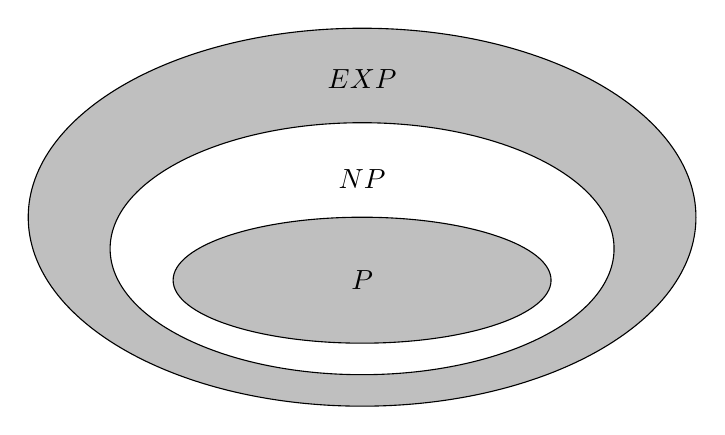
\begin{tikzpicture}[scale=0.8]
      \draw[fill=lightgray] (0,1) ellipse (5.3 and 3);
      \draw[fill=white] (0,0.5) ellipse (4 and 2);
      \draw[fill=lightgray] (0,0) ellipse (3 and 1);
      \node at (0,0) {$P$};
      \node at (0,1.6) {$NP$};
      \node at (0,3.2) {$EXP$};
  \end{tikzpicture}
  \end{center}
  \end{theorem}
  \begin{proof}
  Suppose that $F \in \mathbf{P}$. Define the following function $V$:
  \[V (x 0^n) = \begin{cases}
  1 & \text{iff } n = |x|, F(x) = 1 \\
  0 & \text{else} 
  \end{cases}\]
  Since $F \in \mathbf{P}$, we can clearly compute $V$ in polynomial time as well. Let $x \in \{0,1\}^n$ be some string. If $F(x) = 1$ then $V(x 0^n) = 1$. On the other hand, if $F(x) = 0$ then for every $w \in \{0,1\}^n$, $V(xw) = 0$. Therefore, setting $a = 1$ (i.e. $w \in \{0,1\}^{n^1}$), we see that $V$ satisfies the NP condition. 
  \end{proof}

\subsection{NP Hard and NP Complete Problems}

  There are countless examples of problems for which we do not know if their best algorithm is polynomial or exponential, but we can show that they are in \textbf{NP}; that is, we don't know if they are easy to \textit{solve}, but we do know that it is easy to \textit{verify} a given solution. There are many other functions that we would like to compute that are easily shown to be in \textbf{NP}. In fact, it we can solve 3SAT then we can solve all of them! 

  \begin{theorem}[Cook-Levin Theorem]
  For every $F \in \mathbf{NP}$, 
  \[F \leq_p 3SAT\]
  \end{theorem}
  This immediately implies that $QUADEQ, LONGPATH$, and $MAXCUT$ (and really, \textit{every} $F \in \mathbf{NP}$) all reduce to $3SAT$, meaning that all these problems are equivalent! All of these problems are the "hardest in \textbf{NP}" since an efficient algorithm for any one of them would imply an efficient algorithm for \textit{all} the problems in \textbf{NP}. 

  \begin{definition}
  Let $G: \{0,1\}^* \longrightarrow \{0,1\}$. We say that $G$ is \textbf{NP hard} if for every $F \in \mathbf{NP}$, $F \leq_p G$. We say that $G$ is \textbf{NP complete} if $G$ is \textbf{NP} hard and $G \in \mathbf{NP}$. 
  \end{definition}

  Therefore, despite their differences, 3SAT, quadratic equations, longest path, independent set, maximum cut, and thousands of other problems are all \textbf{NP} complete. Again, this means that \textit{if a single \textbf{NP} complete problem has a polynomial-time algorithm, then there is such a polynomial-time algorithm for every decision problem that corresponds to the existence of an efficiently verifiable solution (i.e. is NP), which would imply that \textbf{P = NP}}.

\subsection{P = NP?}

  However, a polynomial-time algorithm for even a single one of the \textbf{NP} complete problems has even been found, proving support that \textbf{P $\neq$ NP}

  One of the mysteries of computation is that people have observed a certain empirical “zero-one law” or “dichotomy” in the computational complexity of natural problems, in the sense that many natural problems are either in \textbf{P} (often in $TIME(O(n))$ or $TIME(O(n^2))$), or they are \textbf{NP} hard. This is related to the fact that for most natural problems, the best known algorithm is either exponential or polynomial, rather than any strange function in between. 

  However, it is believed that there exist problems in \textbf{NP} that are neither in \textbf{P} nor are \textbf{NP} complete, and in fact a result known as \textbf{Lander's Theorem} shows that if $\mathbf{P \neq NP}$, then this is indeed the case. Therefore, we are left with two cases:
  \begin{enumerate}
      \item If $\mathbf{P} \neq \mathbf{NP}$, meaning that \textbf{P} is a strict subset of \textbf{NP} and by Lander's theorem, \textbf{NP} complete problems do not cover all of $\mathbf{NP} \setminus \mathbf{P}$. (left)
      \item If $\mathbf{P} = \mathbf{NP}$, meaning that $\mathbf{P} = \mathbf{NP} = \mathbf{NP}$ complete. (right)
  \end{enumerate}
  \begin{center}
  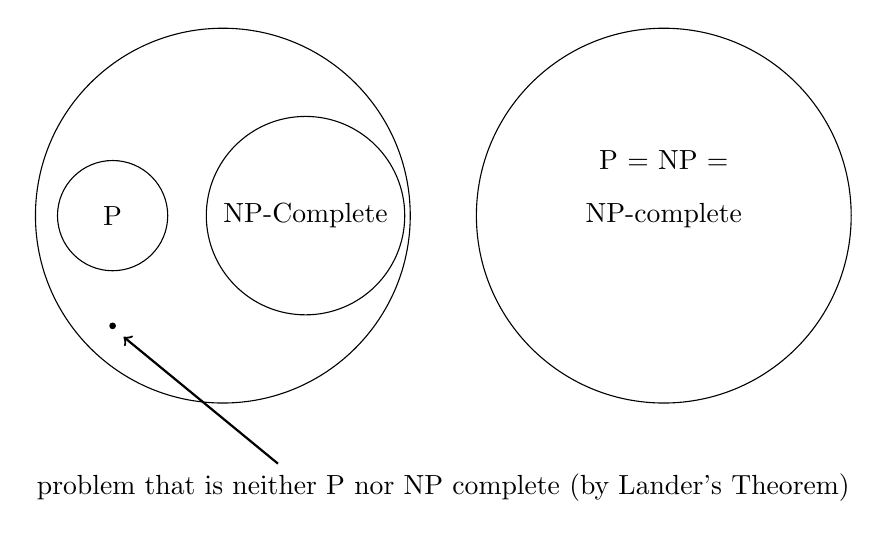
\begin{tikzpicture}[scale=0.7]
      \draw (-4, 0) circle (3.4);
      \draw (4, 0) circle (3.4);
      \draw (-6, 0) circle (1);
      \node at (-6,0) {P};
      \draw (-2.5, 0) circle (1.8);
      \node at (-2.5,0) {NP-Complete};
      \node at (4, 1) {P = NP = };
      \node at (4, 0) {NP-complete};
      \draw[fill] (-6, -2) circle (0.05);
      \draw[->, thick] (-3, -4.5)--(-5.8,-2.2);
      \node[below] at (0, -4.5) {problem that is neither P nor NP complete (by Lander's Theorem)};
  \end{tikzpicture}
  \end{center}

\subsection{NANDSAT, 3NAND Problems}

  \begin{definition}
  The function $NANDSAT: \{0,1\}^* \longrightarrow \{0,1\}$ is defined as follows: 
  \begin{enumerate}
      \item The input to $NANDSAT$ is a string $Q$ representing a NAND-CIRC program (or equivalently, a circuit with $NAND$ gates)
      \item The output of $NANDSAT$ on input $Q$ is $1$ if and only if there exists a string $w \in \{0,1\}^n$ (where $n$ is the number of inputs to $Q$) such that $Q(w) = 1$. 
  \end{enumerate}
  \end{definition}

  \begin{definition}
  The $3NAND$ problem is defined as follows: 
  \begin{enumerate}
      \item The input is a logical formula $\Psi$ on a set of variables $z_0, ..., z_{r-1}$ which is an AND of constraints of the form $z_i = NAND(z_j, z_k)$. 
      \item The output is $1$ is and only if there is an input $z \in \{0, 1\}^r$ that satisfies all of the constraints. 
  \end{enumerate}
  \end{definition}

  \begin{example}
  The following is a $3NAND$ formula with $5$ variables and $3$ constraints:
  \[\Psi = \big( z_3 = NAND(z_0, z_2)\big) \wedge \big( z_1 = NAND(z_0, z_2)\big) \wedge \big( z_4 = NAND(z_3, z_1)\big)\]
  In this case $3NAND(\Psi) = 1$, since the assignment $z = 01010$ satisfies it. Given a $3NAND$ formula $\Psi$ of $r$ variables and an assignment $z \in \{0,1\}^r$, we can check in polynomial time whether $\Psi (z) = 1$, and hence $3NAND \in \mathbf{NP}$. 
  \end{example}

  \begin{theorem}
  $NANDSAT$ and $3NAND$ is \textbf{NP} complete. 
  \end{theorem}

